% fft2.svg 的 TikZ 矢量源：单位圆与特殊角（弧度 / 角度 / 坐标）
% 编译：latex fft2.tex && dvisvgm --exact --no-fonts --precision=8 fft2.dvi
\def\pgfsysdriver{pgfsys-dvisvgm.def}
\documentclass[tikz,border=2pt]{standalone}
\usepackage{amsmath}
\usetikzlibrary{arrows.meta}
\pagecolor{white}
\begin{document}
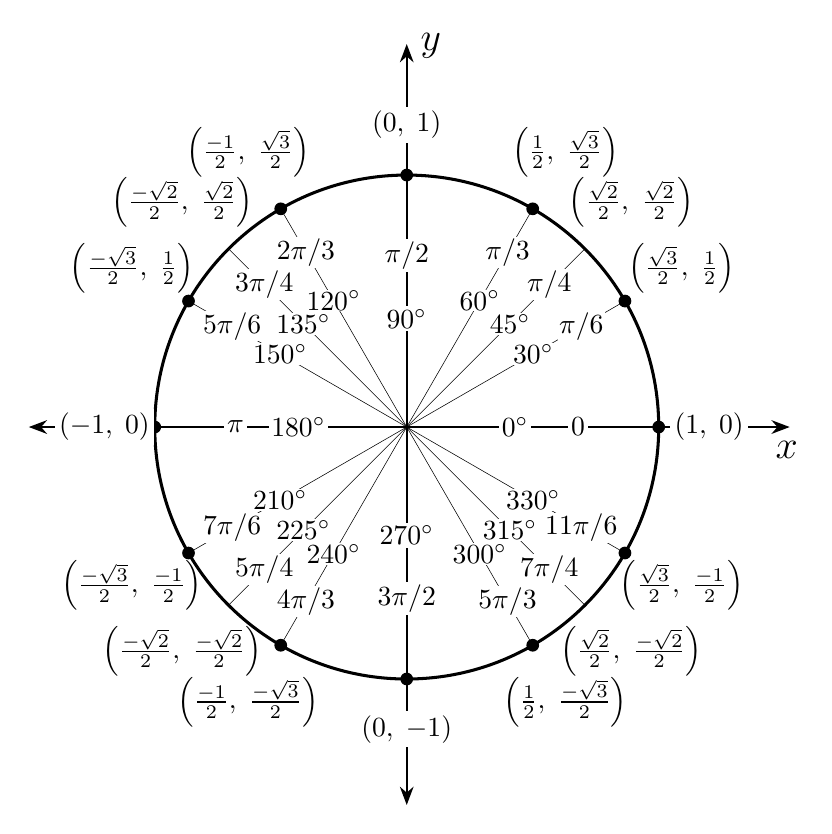
\begin{tikzpicture}[>=Stealth,line cap=round,line join=round]
  \def\R{3.2}
  % 单位圆
  \draw[line width=1.1pt] (0,0) circle[radius=\R];
  % 坐标轴
  \draw[line width=0.8pt,<->] (-1.5*\R,0) -- (1.52*\R,0);
  \draw[line width=0.8pt,<->] (0,-1.5*\R) -- (0,1.52*\R);
  \node[anchor=south west,inner sep=2pt] at (0.1,1.44*\R) {\Large $y$};
  \node[anchor=north west,inner sep=2pt] at (1.44*\R,-0.1) {\Large $x$};
  % 12 条非坐标轴方向的射线
  \foreach \a in {30,45,60,120,135,150,210,225,240,300,315,330}
    \draw[very thin] (0,0) -- (\a:\R);
  % 16 个分点
  \foreach \a in {0,30,...,330}
    \fill (\a:\R) circle[radius=2.3pt];
  % 圆内标注：弧度（靠外）与角度（靠内）
  \foreach \a/\rad/\degs in {
    30/{\pi/6}/{30^\circ},45/{\pi/4}/{45^\circ},60/{\pi/3}/{60^\circ},
    120/{2\pi/3}/{120^\circ},135/{3\pi/4}/{135^\circ},150/{5\pi/6}/{150^\circ},
    210/{7\pi/6}/{210^\circ},225/{5\pi/4}/{225^\circ},240/{4\pi/3}/{240^\circ},
    300/{5\pi/3}/{300^\circ},315/{7\pi/4}/{315^\circ},330/{11\pi/6}/{330^\circ}}{
    \node[fill=white,inner sep=0.5pt] at (\a:0.80*\R) {$\rad$};
    \node[fill=white,inner sep=0.5pt] at (\a:0.58*\R) {$\degs$};
  }
  % 坐标轴上的四组标注
  \node[fill=white,inner sep=1pt] at (0.68*\R,0)  {$0$};
  \node[fill=white,inner sep=1pt] at (0.43*\R,0)  {$0^\circ$};
  \node[fill=white,inner sep=1pt] at (0,0.68*\R)  {$\pi/2$};
  \node[fill=white,inner sep=1pt] at (0,0.43*\R)  {$90^\circ$};
  \node[fill=white,inner sep=1pt] at (-0.68*\R,0) {$\pi$};
  \node[fill=white,inner sep=1pt] at (-0.43*\R,0) {$180^\circ$};
  \node[fill=white,inner sep=1pt] at (0,-0.68*\R) {$3\pi/2$};
  \node[fill=white,inner sep=1pt] at (0,-0.43*\R) {$270^\circ$};
  % 圆外坐标标注（斜方向）
  \foreach \a/\nx/\dx/\ny/\dy in {
    30/{\sqrt3}/{2}/{1}/{2},45/{\sqrt2}/{2}/{\sqrt2}/{2},60/{1}/{2}/{\sqrt3}/{2},
    120/{-1}/{2}/{\sqrt3}/{2},135/{-\sqrt2}/{2}/{\sqrt2}/{2},150/{-\sqrt3}/{2}/{1}/{2},
    210/{-\sqrt3}/{2}/{-1}/{2},225/{-\sqrt2}/{2}/{-\sqrt2}/{2},240/{-1}/{2}/{-\sqrt3}/{2},
    300/{1}/{2}/{-\sqrt3}/{2},315/{\sqrt2}/{2}/{-\sqrt2}/{2},330/{\sqrt3}/{2}/{-1}/{2}}{
    \node[inner sep=1.5pt] at (\a:1.26*\R)
      {$\left(\frac{\nx}{\dx},\;\frac{\ny}{\dy}\right)$};
  }
  % 圆外坐标标注（轴向）
  \node[fill=white,inner sep=1.5pt] at (1.20*\R,0)   {$(1,\;0)$};
  \node[fill=white,inner sep=1.5pt] at (0,1.20*\R)   {$(0,\;1)$};
  \node[fill=white,inner sep=1.5pt] at (-1.20*\R,0)  {$(-1,\;0)$};
  \node[fill=white,inner sep=1.5pt] at (0,-1.20*\R)  {$(0,\;-1)$};
\end{tikzpicture}
\end{document}
